\section{End-to-End Pipeline}

The pipeline connects the datasets and splits discussed in Section~\ref{sec:datasets_and_splits} with the experimental protocol defined in Section~\ref{sec:experimental_protocol}. Its role is to transform raw datasets into a common representation and then use that representation to train, select, evaluate, and analyze the models in a reproducible way.

The implemented workflow is organized into five main stages: (i) manifest generation, where raw dataset folders are converted into comma-separated values (CSV) manifests; (ii) offline preprocessing, where images are deterministically processed once, updated manifests are written, and dataset-level statistics are computed; (iii) experiment execution, where configuration files are expanded into concrete runs and the framework performs online data augmentation, training, validation-based model selection, checkpointing, logging, and optional test evaluation; (iv) log parsing and aggregation, where the resulting JSON Lines (JSONL) logs are used to build rankings and aggregate validation or test metrics; and (v) qualitative example export, where selected checkpoints are restored to produce visual examples for inspection.

Figure~\ref{fig:pipeline} summarizes the implemented workflow and shows how the dataset preparation stages are connected to experiment execution, log aggregation, and qualitative analysis.

\begin{figure*}[t]
    \centering
    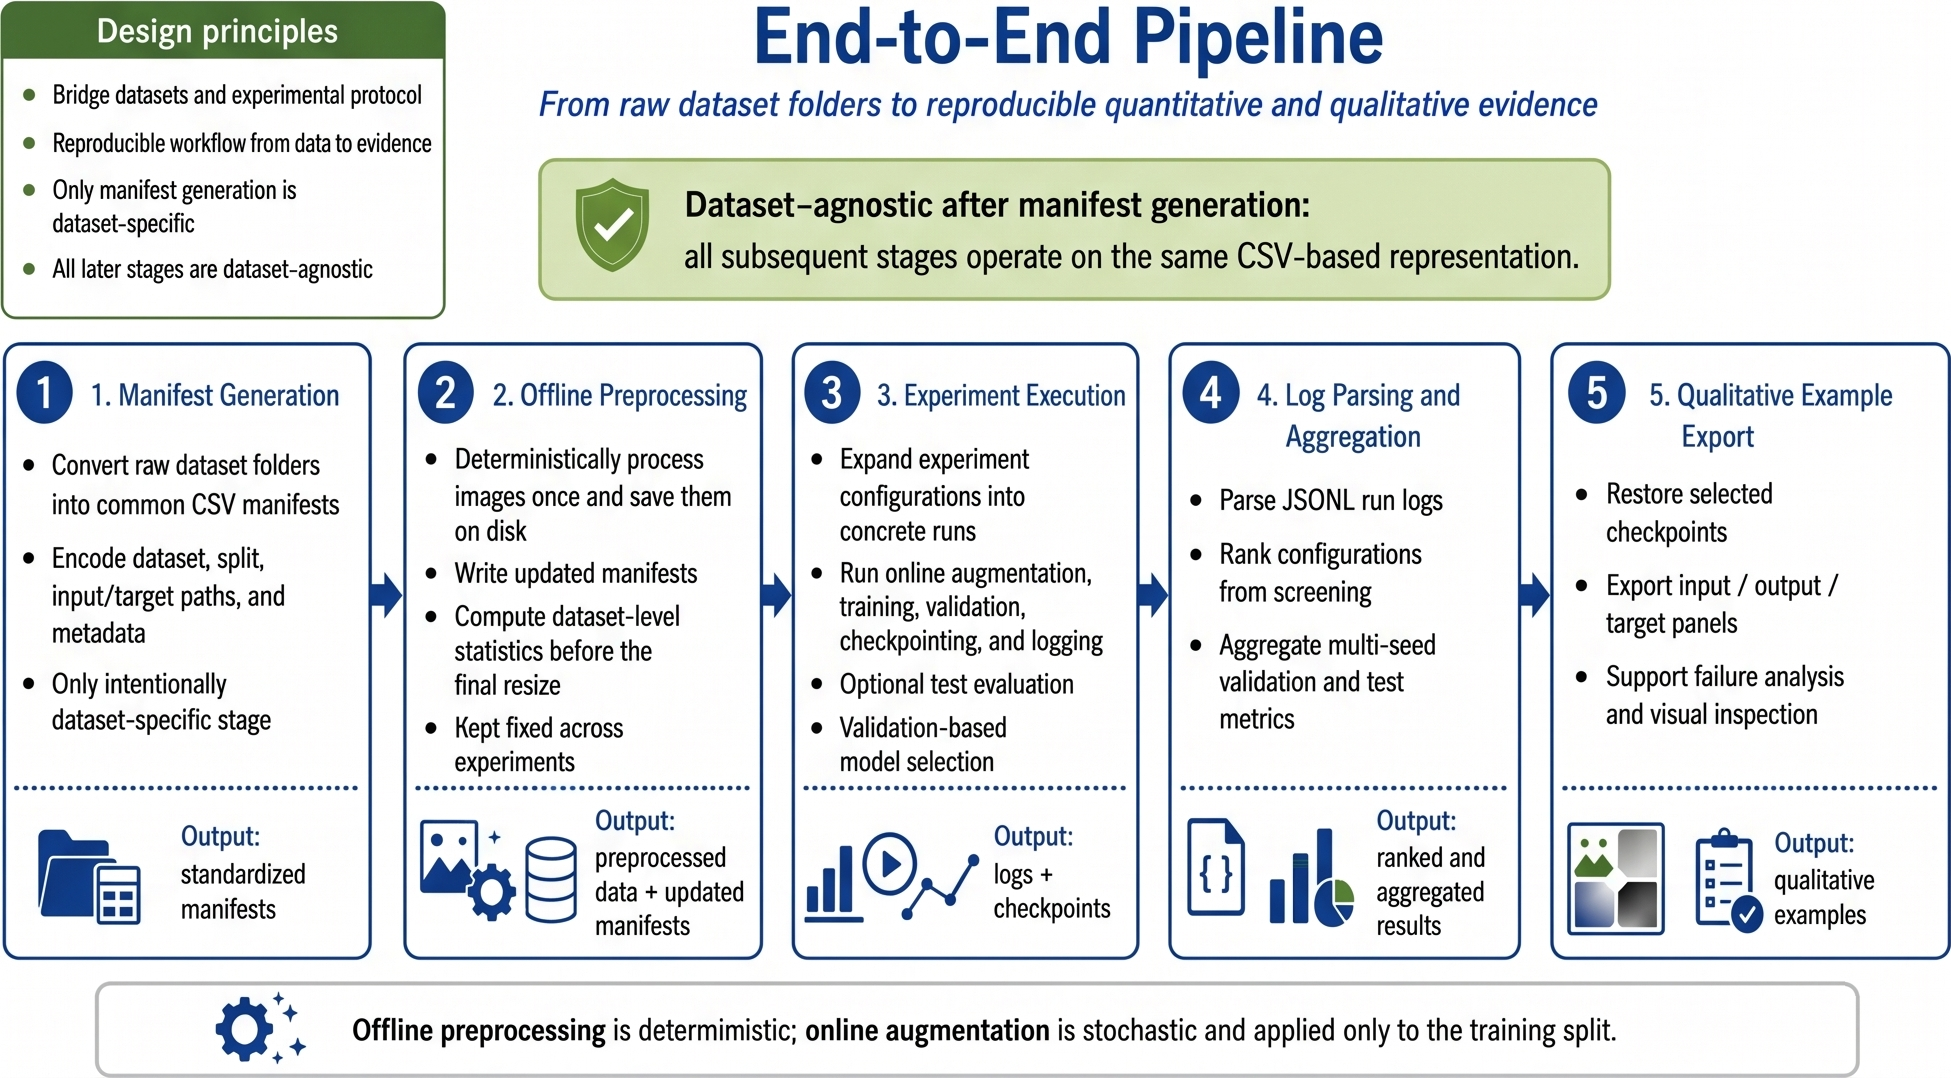
\includegraphics[width=\textwidth]{fig/pipeline/pipeline.png}
    \caption{Overview of the end-to-end pipeline.}
    \label{fig:pipeline}
\end{figure*}

``Offline'' preprocessing and ``online'' augmentation serve different purposes in the pipeline. Offline preprocessing consists of deterministic operations that are performed once before training, saved on disk, and kept fixed across experiments. Online augmentation is instead applied at training time, when samples are loaded from the training split, and has a stochastic nature because the transformations are randomly sampled during training. In the current configuration, geometric augmentations are applied consistently to both the low-light input and the paired target, while photometric perturbations are applied only to the input image. This preserves the alignment of paired samples while exposing the model to additional low-light variations.

The pipeline follows a central design principle of the project: only the manifest generation stage is intentionally dataset-specific. This stage absorbs the differences between the original dataset structures, such as pairing rules, filename conventions, category folders, and illumination-level metadata. Once each dataset has been converted into the CSV manifest format, the following stages of the pipeline operate on the same representation and do not need to know how each dataset was originally organized on disk.

The following subsections describe these stages in more detail, showing how each part of the pipeline is implemented in the codebase.

\subsection{Manifest Generation}
\label{sec:manifest_generation}

The purpose of the first stage of the pipeline is to scan the original dataset folders and build CSV manifest files from their structure. In each manifest, every row represents one image sample and stores the dataset name, the split to which the sample belongs, the path of the low-light input image, the path of the corresponding target image when available, and optional metadata such as image category or illumination level.

This step is necessary because the datasets used in this project are not organized in the same way. Some provide paired low-light and normal-light images with the same filename, while others use different filename conventions. ExDark is instead unpaired and organized by object category. MILLs also includes an illumination level in the input filename, which is useful for analyzing how performance changes under different lighting conditions. Without this standardization, subsequent pipeline scripts would need to include several dataset-specific rules.

For this reason, manifest generation is the only intentionally dataset-specific part of the pipeline. The script reads a YAML configuration file describing dataset locations, output files, and the rules used to create each manifest. In LOL-v2 Real, filenames differ only because low-light and reference images use different prefixes. In LOL-v2 Synthetic, low-light images and their corresponding reference images share the same filename, making the association straightforward. In MILLs, the filename also contains the illumination level, which is extracted and stored together with the path of the corresponding reference image. ExDark follows a different structure: images are grouped by category and no reference image is available, so only the image path and category information are recorded. Finally, LOL-v1 is handled as a paired overlap-control set; its low-light images and corresponding reference images also share the same filename.

The output of this step is a CSV manifest file for each dataset, with a fixed column structure. This common format makes the later stages dataset-agnostic: once the manifests are created, preprocessing, training, and evaluation only need to read the paths and metadata stored in the CSV files, without knowing how the original datasets are arranged on disk.

Manifest generation also includes reproducibility measures. When required by the protocol and a training split is available, a validation split is sampled from it using a fixed seed. Rows are sorted by split and image path, ensuring deterministic order across runs.

The manifest metadata supports evaluation: MILLs illumination levels enable global and per-level results, while ExDark categories enable global and per-category reporting. Evaluation remains general while retaining metadata for analysis.

\subsection{Offline Preprocessing}

\analysispar{Deterministic preprocessing}
After manifest generation, all datasets are processed by an offline preprocessing script. This stage is called ``offline'' because it contains deterministic preliminary operations that are performed once for all the experiments of this project rather than repeatedly during training or evaluation. The processed images are stored on disk and are then used by all later stages of the pipeline.

For each CSV manifest, the script first performs a lightweight consistency check. It verifies that no input path is duplicated within the same split and that the same input path does not appear in different splits. These checks are intentionally limited, since the dataset-specific pairing rules have already been handled during manifest generation.

After these checks, the script creates a preprocessed version of each dataset on disk. For each dataset, it also writes a new CSV manifest with the same columns as the original one, but with paths updated to the preprocessed images. The output paths preserve the dataset-relative folder structure of the original files, while the image extension is replaced according to the selected output format.

Each image undergoes the following deterministic operations: (i) loading with Exchangeable Image File Format (EXIF) orientation applied when available, (ii) conversion to RGB, (iii) resizing to $256 \times 256$ using Lanczos interpolation, and (iv) saving in Portable Network Graphics (PNG) format. Applying the EXIF orientation avoids processing photographs with an incorrect rotation. PNG is used to avoid introducing additional compression artifacts during preprocessing. If the same source image is referenced more than once in a manifest, it is processed only once and then reused, avoiding possible duplicated work.

A fixed resizing strategy is used instead of cropping. In this project, preserving the whole scene during preprocessing was considered preferable to selecting a local region, because a crop would permanently discard part of the image and could remove relevant low-light regions, light sources, or objects needed for cross-dataset analysis. Although resizing may slightly distort the aspect ratio of some images, it keeps the full scene and provides a fixed deterministic input size for all datasets. This choice does not exclude the use of cropping as online data augmentation during training: unlike offline cropping, random resized crops are stochastic, do not permanently modify the preprocessed dataset, and are applied only to the training split, while validation and test images remain deterministic.

\analysispar{Dataset statistics}
Besides producing preprocessed images and updated manifests, the script computes dataset-level statistics and writes them to a dedicated summary file. These are calculated before final resizing, after loading each image with the correct orientation and converting it to RGB. They therefore describe original image sizes and illumination properties before conversion to fixed $256 \times 256$ dimensions.

For each image of size $H \times W$, a luminance map $Y \in [0,1]^{H \times W}$ is computed from the RGB channels using the ITU-R BT.709 luma coefficients:
\begin{equation}
	Y_{i,j} = 0.2126R_{i,j} + 0.7152G_{i,j} + 0.0722B_{i,j},
	\label{eq:luminance}
\end{equation}
where $R_{i,j}$, $G_{i,j}$, and $B_{i,j}$ are the RGB values of pixel $(i,j)$, scaled to $[0,1]$. Based on this luminance map, the dark pixel ratio (DPR) is defined as
\begin{equation}
	\mathrm{DPR}
	=
	\frac{1}{HW}
	\sum_{i=1}^{H}
	\sum_{j=1}^{W}
	1\left[Y_{i,j} < \tau_d\right],
	\label{eq:dpr}
\end{equation}
where $H$ and $W$ are the image height and width respectively, $\tau_d = 0.10$ is the dark-pixel threshold, and $1[\cdot]$ is the indicator function, equal to one when the condition is true and zero otherwise.

For each dataset, the script records the number of samples, the median original input size, the mean and standard deviation of input luminance, and the average fraction of dark pixels. For paired datasets, the same luminance summary is also computed on the target images. These statistics are written to a dataset summary file and are reported in Table~\ref{tab:dataset_statistics}.

\begin{table*}[t]
	\centering
	\caption{Dataset statistics computed during offline preprocessing, before applying the final resize. The first row reports the main dataset, while LOL-v2 Synthetic, MILLs, and ExDark are independent external evaluation datasets. LOL-v1 (overlap) is retained as a non-independent descriptive control and is excluded from independent cross-dataset conclusions. Luminance values are reported as mean $\pm$ standard deviation across samples. Target luminance is not available for ExDark because it is unpaired.}
	\label{tab:dataset_statistics}
	\begin{tabular}{lccccc}
		\toprule
		Dataset & Samples & Median original size (px) & Input luminance & Dark pixels (\%) & Target luminance \\
		\midrule
		LOL-v2 Real & 789 & $600 \times 400$ & $0.062 \pm 0.042$ & $80.9$ & $0.436 \pm 0.105$ \\
		\midrule
		LOL-v2 Synthetic & 1000 & $384 \times 384$ & $0.240 \pm 0.138$ & $46.7$ & $0.513 \pm 0.141$ \\
		MILLs & 499 & $600 \times 400$ & $0.244 \pm 0.110$ & $16.4$ & $0.369 \pm 0.095$ \\
		ExDark & 7363 & $640 \times 500$ & $0.143 \pm 0.086$ & $59.6$ & -- \\
		\midrule
		LOL-v1 (overlap) & 500 & $600 \times 400$ & $0.061 \pm 0.041$ & $82.7$ & $0.458 \pm 0.102$ \\
		\bottomrule
	\end{tabular}
\end{table*}

The statistics provide a compact description of the illumination distribution encountered by the preprocessing pipeline. LOL-v2 Synthetic and MILLs are brighter on average, indicating a larger distribution shift in terms of illumination. ExDark lies between these cases in terms of input luminance and remains useful as an unpaired real-world stress test. Finally, LOL-v1 has an input luminance distribution nearly identical to LOL-v2 Real, as expected from its overlap-control relationship.

\subsection{Experiment Execution}
\label{sec:experiment_execution}

\analysispar{Run configuration}
After offline preprocessing, the third stage of the pipeline is experiment execution. This stage uses the preprocessed manifests to run the experiments required by the protocol. It is model-agnostic: the pipeline does not assume a specific architecture. Instead, each run is built from an experiment configuration, which specifies the model family, the training and validation manifests, the hyperparameters, the loss function, the online data augmentation policy, the early-stopping rule, and whether test evaluation should be executed.

The experiment launcher expands the hyperparameter grid defined in the configuration and creates one resolved configuration for each combination of values, i.e., a set of configurations in which every grid parameter has been replaced by one concrete value. This makes it possible to describe a large set of experiments compactly.

Each resolved configuration is assigned a configuration identifier. This identifier is computed from the part of the configuration that defines the model and its training setup, while run-specific or evaluation-specific fields are ignored. In this way, repeated runs of the same configuration, for example with different seeds, can be recognized and aggregated correctly.

\analysispar{Training, data augmentation, and validation}
For each run, the framework builds the model, the loss function, the optimizer, and the data loaders from the resolved configuration. Model-specific details are isolated behind lightweight model-family wrappers, which define how the model and loss are constructed, how a batch is passed through the model, and how the model output is interpreted as a prediction. Training and validation samples are read from the preprocessed manifests, using the split field to distinguish the two partitions. Since at this point of the pipeline the input format is the same for all datasets, the execution stage no longer depends on the original dataset folder structure.

The optimizer used in the experiments is AdamW~\cite{DBLP:conf/iclr/LoshchilovH19}. This choice keeps the practical advantages of Adam-based optimization, such as adaptive learning rates and stable training for convolutional image-to-image models, while using a more explicit form of weight regularization. This is useful in this project because weight decay is part of the optimization search space and is intended to reduce overfitting to the LOL-v2 Real training distribution. Compared with standard Adam with coupled L2 regularization, AdamW decouples weight decay from the adaptive gradient update, making the regularization effect cleaner and easier to control. This is especially relevant in a cross-dataset protocol, where the goal is not only to fit the source dataset, but also to preserve generalization under distribution shift.

Online data augmentation is also part of experiment execution. The augmentation policy is defined in the experiment configuration and can enable or disable each transformation and control its sampling behavior. In the current experimental protocol, however, this policy is kept fixed across runs, so that model configurations are compared under the same data variability.

Augmentation is applied only to samples loaded from the training split. The framework explicitly prevents it from being enabled for validation or test splits, so validation and test metrics are always computed on deterministic preprocessed images. The augmentation pipeline is applied after reading the preprocessed RGB images and before converting them to tensors.

The transformations are considered in a fixed order: (i) horizontal flipping, (ii) random resized cropping, (iii) color jitter, (iv) gamma jitter, and (v) additive synthetic sensor noise. When enabled, random resized cropping is applied to each training sample by randomly sampling the crop parameters. The other stochastic transformations are applied according to their configured probabilities. Therefore, a training sample does not always receive the full sequence of transformations: depending on the random decisions, different samples can undergo different combinations of augmentations. This creates a wide variety of possible augmented inputs while keeping the augmentation policy fixed across experiments.

Each transformation has a specific role. Horizontal flipping exposes the model to mirrored versions of the same scene. Random resized cropping changes the visible region and slightly varies the scale of the content. Color jitter perturbs brightness, contrast, and saturation, while gamma jitter modifies the brightness curve of the input image, affecting dark and bright regions differently. Finally, synthetic sensor noise adds small random perturbations to simulate noisy low-light acquisitions.

Horizontal flipping and random resized cropping are geometric transformations. They are applied consistently to both the low-light input and the paired target, using the same random decision and the same spatial parameters. This preserves the pixel-level alignment required by supervised training. Color jitter, gamma jitter, and synthetic sensor noise are photometric perturbations. They are applied only to the low-light input, because their purpose is to simulate additional low-light variability without modifying the reference image. This distinction allows the model to see a broader range of degraded inputs while keeping the target image as a stable normally exposed reference.

Online augmentation improves generalization by exposing the model to plausible variations of training images. Without it, the model could overfit the framing, scale, color distribution, gamma response, and noise pattern of LOL-v2 Real. Geometric transformations reduce sensitivity to spatial arrangement, while photometric perturbations simulate changes in camera response, exposure, color, and sensor noise. This is particularly important in cross-dataset evaluation, where test data may differ in scene content, acquisition conditions, and low-light statistics.

Training is performed on paired samples. The model receives the low-light input image and predicts an enhanced RGB image. The loss function then compares this prediction with the corresponding reference image according to the objective specified in the configuration. At the configured validation interval, the framework evaluates the model on the validation split, computes the configured validation metrics, updates the early-stopping state, and stores the model state when a new best validation result is obtained.

Before being passed to the model, training images are converted to tensors after online augmentation, while validation images are converted directly after loading because validation is not augmented. In both cases, image tensors are represented with values in the normalized range $[0, 1]$. This convention is used consistently for low-light inputs, reference targets, model predictions, paired losses, full-reference metrics, and diagnostic metrics. Using a normalized image range keeps the numerical scale of the training objective controlled and makes quantities such as MAE, luminance statistics, dark-pixel thresholds, clipping thresholds, and RGB imbalance directly interpretable. It also matches the output design of the enhancement models, which constrain their predictions to the same valid image range through bounded output operations such as sigmoid activations or final clipping. This avoids producing values outside the expected intensity interval and ensures that losses and metrics compare prediction and target under the same convention.

For reproducibility, the paired quantities used during training and validation are defined below. Given a prediction $\hat{I}$ and a target image $I$, both with $C$ channels and spatial size $H \times W$, the MAE is computed as
\begin{equation}
	\mathrm{MAE}(\hat{I}, I)
	=
	\frac{1}{CHW}
	\sum_{c=1}^{C}
	\sum_{i=1}^{H}
	\sum_{j=1}^{W}
	\left|
	\hat{I}_{c,i,j} - I_{c,i,j}
	\right|.
	\label{eq:mae}
\end{equation}
The same expression can also be used as an L1 loss term during training when selected by the configuration.

SSIM compares prediction and target images in terms of local luminance, contrast, and structure. It is computed independently for each channel using a local averaging window:
\begin{equation}
	\mathrm{SSIM}(\hat{I}, I)
	=
	\frac{
		(2\mu_{\hat{I}}\mu_I + C_1)
		(2\sigma_{\hat{I}I} + C_2)
	}{
		(\mu_{\hat{I}}^2 + \mu_I^2 + C_1)
		(\sigma_{\hat{I}}^2 + \sigma_I^2 + C_2)
	},
	\label{eq:ssim}
\end{equation}
where $\mu_{\hat{I}}$ and $\mu_I$ are the local means, and $\sigma_{\hat{I}}^2$ and $\sigma_I^2$ are the local variances of the prediction $\hat{I}$ and the reference image $I$, respectively; $\sigma_{\hat{I}I}$ is their local covariance. The constants $C_1$ and $C_2$ are small stabilization constants used to avoid numerical instability when local means or variances are close to zero. The final SSIM value is obtained by averaging the local SSIM values over all spatial positions and channels.

PSNR is derived from the mean squared error (MSE), which measures the average squared difference between the prediction and reference image. The MSE is defined as
\begin{equation}
	\mathrm{MSE}(\hat{I}, I)
	=
	\frac{1}{CHW}
	\sum_{c=1}^{C}
	\sum_{i=1}^{H}
	\sum_{j=1}^{W}
	\left(
	\hat{I}_{c,i,j} - I_{c,i,j}
	\right)^2,
	\label{eq:mse}
\end{equation}
and PSNR is then computed as
\begin{equation}
	\mathrm{PSNR}(\hat{I}, I)
	=
	10 \log_{10}
	\left(
	\frac{1}{\max(\mathrm{MSE}(\hat{I}, I), 10^{-10})}
	\right).
	\label{eq:psnr}
\end{equation}
The small lower bound inside the maximum avoids numerical instability when the MSE is extremely close to zero.

During validation, the framework computes the loss and the full-reference metrics on the validation split. No-reference and diagnostic metrics are skipped at this stage, because they are not used for checkpoint selection and would make the validation loop heavier.

Early stopping is configured in a model-agnostic way. The framework monitors a primary validation metric and can use a secondary validation metric as a tie-breaker when the primary metric changes by less than the configured tolerance. When the number of consecutive non-improving validation steps reaches the patience value, training stops.

Mixed precision is controlled by the experiment configuration. When enabled, it allows some training computations to use lower numerical precision, which can reduce memory usage and improve speed. This option is used only when a CUDA device, namely an NVIDIA graphics processing unit (GPU), is available. In that case, the framework also uses a gradient scaler: it temporarily multiplies the loss by a scaling factor before backpropagation, so that very small gradients are easier to represent in lower precision, and then scales the gradients back before the optimizer updates the model weights. This helps reduce numerical instability while still benefiting from mixed precision. If mixed precision is disabled or CUDA is not available, training is performed in standard precision.

\analysispar{Logging and checkpointing}
For each run, the framework writes a JSONL log, in which every line is a separate JSON object. Each resolved run is written to a separate JSONL file inside an experiment-specific log directory, so that later parsing scripts can process runs independently and aggregate them by configuration. This format is useful because later parsers can read the logs line by line and extract only the events needed for ranking, aggregation, or reporting. The first log event stores general information about the run, including the resolved configuration, the random seed, the device, the checkpoint location, and the total number of model parameters. More specifically, the number of parameters is computed as the sum of all tensor elements in the model parameters, and it can later be used to compare configurations not only in terms of validation performance, but also in terms of model size.

Each run also saves a checkpoint containing both the model weights and the additional information needed to resume or reuse the run. This file includes the current and best validation model weights, optimizer information, the mixed-precision scaler when applicable, training and early-stopping information, random generator states, and the resolved configuration. Therefore, the same checkpoint can be used to resume training, restore the best validation model for test evaluation, or export qualitative examples.

\analysispar{Test evaluation}
When test evaluation is enabled in the experiment configuration file, it is also executed inside this stage of the pipeline. Before evaluation starts, the framework restores the best model state selected on the validation set by early stopping.

The evaluator loops over the configured test manifests and computes global metrics over all samples. If the manifest contains a grouping field requested by the configuration, the evaluator also computes grouped metrics. This is how the same evaluation code supports category-level reporting for ExDark and illumination-level reporting for MILLs.

The evaluator automatically adapts to paired and unpaired datasets. If a target image is available in the preprocessed CSV manifest, full-reference metrics are computed. These include SSIM, PSNR, and MAE. If the target path is empty, full-reference metrics are skipped. No-reference metrics and diagnostic metrics are computed only from the enhanced output image and can therefore be used for both paired and unpaired datasets.

The no-reference metrics NIQE and BRISQUE are not implemented explicitly. They are computed through the \texttt{pyiqa} library, using the corresponding metric objects provided by the library.

Diagnostic metrics are computed on the enhanced output $\hat{I}$. The output luminance map $\hat{Y}$ is computed with the same BT.709 definition introduced during offline preprocessing in Eq.~\ref{eq:luminance}, but it is applied to the model output rather than to the original input image. From this map, the framework derives three output-level summaries: mean luminance, luminance standard deviation, and dark pixel ratio. Mean luminance and dark pixel ratio help detect residual darkness or excessive brightening, while luminance standard deviation provides a compact indication of contrast variation. The dark pixel ratio uses the same threshold-based definition in Eq.~\ref{eq:dpr}, again applied to $\hat{Y}$.

The bright clipping ratio (BCR) is used to detect possible over-exposure. It measures the fraction of pixels for which at least one RGB channel is close to saturation:
\begin{equation}
	\mathrm{BCR}
	=
	\frac{1}{HW}
	\sum_{i=1}^{H}
	\sum_{j=1}^{W}
	1
	\left[
	\max_{c \in \{R,G,B\}}
	\hat{I}_{c,i,j} > \tau_b
	\right],
	\label{eq:bcr}
\end{equation}
where $\tau_b = 0.98$ is the bright-clipping threshold. Together with mean luminance, this metric helps distinguish globally bright outputs from outputs that contain localized saturated regions.

The RGB channel imbalance (RGBI) is used as a simple indicator of color cast. It compares the mean values of the three output channels and measures the gap between the largest and smallest one:
\begin{equation}
	\mathrm{RGBI}
	=
	\max_{c \in \{R,G,B\}} \mu_c
	-
	\min_{c \in \{R,G,B\}} \mu_c,
	\label{eq:rgbi}
\end{equation}
where $\mu_c$ is the mean value of output channel $c$. A larger value indicates a stronger imbalance between color channels.

Finally, Laplacian sharpness (LS) is used as a simple measure of high-frequency content in the enhanced output. The Laplacian filter highlights rapid changes in the luminance map, such as edges, fine details, noise, or halo artifacts. The metric is the variance of the image obtained after applying the Laplacian kernel:
\begin{equation}
	\mathrm{LS}
	=
	\mathrm{Var}(K \ast \hat{Y}),
	\label{eq:laplacian_sharpness}
\end{equation}
where $\ast$ denotes convolution and
\begin{equation}
	K =
	\begin{bmatrix}
		0 & 1 & 0 \\
		1 & -4 & 1 \\
		0 & 1 & 0
	\end{bmatrix}.
	\label{eq:laplacian_kernel}
\end{equation}
Here, $K$ is the discrete four-neighbour Laplacian kernel. Its positive entries compare each pixel with its vertical and horizontal neighbours, while the negative central coefficient subtracts the current pixel value. Applying this kernel to the output luminance map highlights rapid local changes, such as edges, fine texture, noise, or halo artifacts. Therefore, the variance of the filtered map provides a compact indicator of high-frequency content in the enhanced output. A very low value may indicate over-smoothing or blur, especially when luminance standard deviation is also low. An unusually high value may indicate residual noise, overly sharp edges, or halo artifacts. For halo artifacts, this signal is interpreted together with bright clipping ratio, no-reference quality scores, and visual inspection near light sources and strong edges.

During test evaluation, the framework also logs per-sample metric events. This is useful because global scores summarize average behavior, while individual sample records can later guide qualitative analysis and help identify potential failure cases.

\subsection{Log Parsing and Aggregation}

After experiment execution, the pipeline converts the raw JSONL logs into structured CSV and JSON files. Each run produces a sequence of logged events and, although the JSONL format is convenient during training, it is not directly suitable for analysis because the information is distributed across many event records. Therefore, a dedicated parsing stage reads the logs and reorganizes the relevant information into CSV or JSON files, depending on the type of parsing.

During single-seed screening, each run is summarized by its configuration, number of parameters, best validation epoch, and validation metrics. These summaries are ranked using the validation criterion defined by the experiment, so that the best configurations can be selected for the multi-seed stage. During multi-seed re-training, runs corresponding to the same configuration are grouped together, and the parser computes mean and standard deviation values across seeds, providing a final ranking. This makes it possible to compare configurations not only by average validation performance, but also by their stability.

For final evaluation, the parser aggregates the test metrics of the selected configuration across repeated runs. Results are reported both at dataset-level and, when available, at group-level. More specifically, this allows the same reporting procedure to summarize global results for each test dataset, illumination-level results for MILLs, and category-level results for ExDark. The parsed table preserves full-reference metrics when a paired target is available, and contains only no-reference and diagnostic metrics when no target is provided.

The parsing stage also supports the qualitative analysis. Per-sample evaluation records are first aggregated across repeated runs and then used to build candidate lists for good enhancements and for the main failure types considered in the report. These candidates are selected through metric-based scores computed within each dataset, so that examples are compared against samples from the same distribution. The resulting lists are not treated as final visual evidence automatically; instead, they provide a reproducible pool of examples that is later inspected manually when selecting the qualitative panels.

\subsection{Qualitative Example Export}

The final stage of the pipeline exports qualitative visual examples from the selected checkpoints. This stage is used in two complementary ways. The first one is an intra-family export, where one model family is analyzed in isolation and the goal is to find representative examples of good behavior and failure modes. The second one is an inter-family export, where the selected checkpoints of all model families are applied to the same input images, so that their outputs can be compared directly. This separation supports both failure-oriented inspection and controlled cross-family comparison.

\analysispar{Intra-family export}
The intra-family export uses the sample-level metrics saved during final test evaluation. This is different from the aggregation used for the quantitative tables. During evaluation, each test image first produces its own metric record. Then, the evaluator also averages these records over the whole dataset, and, when required, over groups such as ExDark categories or MILLs illumination levels. These dataset-level and group-level averages are used for the quantitative results, but they are not used to choose the qualitative examples.

For qualitative export, the parser reads the metrics saved for each individual test image. If the same selected model family is evaluated across repeated runs, the records referring to the same image are grouped together. Therefore, each image obtains one aggregated sample record, containing the mean and standard deviation of its own metrics across repeated runs. In this context, ``aggregated'' refers only to the same image across runs, not to all images of a dataset.

For each dataset and for each metric, the script first converts the raw values into relative scores. This means that the images of the same dataset are ordered from the lowest value of that metric to the highest one, so that low values become scores close to $0$ and high values become scores close to $1$. These scores are then used differently depending on the qualitative case that the script is trying to find, namely one of the failure modes or the good-enhancement case. If the selected case is expected to have a high value of a metric, such as many dark pixels for residual darkness, the score is used directly. If it is expected to have a low value of a metric, such as low sharpness for over-smoothing, the score is reversed, so that lower raw values become more important. In this way, all components are transformed so that a higher final score always means a more relevant candidate for the selected qualitative case.

For each image and qualitative category, namely a considered failure type or the good-enhancement case, the script computes a weighted average of the corresponding normalized components. The fixed code-defined weights indicate which diagnostics are more important for that specific case. Samples are then sorted by final score, from most to least relevant, and the ten highest-scoring candidates are retained for each category.

Using the full-reference, no-reference, and diagnostic metrics defined above, the scoring rules ensure that a higher candidate score always indicates a more relevant case.
\begin{itemize}[topsep=5pt]
	\item \textbf{Residual darkness}: the score increases when the dark-pixel ratio is high and the mean luminance is low;
	\item \textbf{Over-exposure}: the score increases when the bright clipping ratio is high and the mean luminance is also high;
	\item \textbf{Color cast}: the score increases when the RGB channel imbalance is high;
	\item \textbf{Over-smoothing}: the score increases when Laplacian sharpness is low and luminance standard deviation is low;
	\item \textbf{Residual noise}: the score increases when NIQE, BRISQUE, and Laplacian sharpness are high;
	\item \textbf{Halo artifacts}: the score increases when bright clipping ratio, Laplacian sharpness, BRISQUE, and NIQE are high;
	\item \textbf{Hallucinated details}: the rule depends on whether the sample is paired. For paired samples, the score increases when SSIM and PSNR are low and MAE is high. For unpaired samples, the score increases when NIQE and BRISQUE are high and when Laplacian sharpness is anomalous;
	\item \textbf{Good enhancement}: this case is selected only for paired samples. The score increases when SSIM and PSNR are high, while MAE, NIQE, BRISQUE, dark-pixel ratio, bright clipping ratio, and RGB channel imbalance are low.
\end{itemize}

Since there are seven failure modes plus the good-enhancement case, this produces eighty exported candidate panels for each model family.

The export script then restores the selected checkpoint of the model, rebuilds the corresponding model wrapper from the saved resolved configuration, loads the best validation model state, and runs inference on the selected candidate images. For each candidate, it saves a visual panel containing the low-light input and the enhanced output. If the sample belongs to a paired dataset, the target image is also added to the panel; if the sample is unpaired, as in ExDark, the panel contains only input and output.

This selection procedure is deliberately approximate. The diagnostic metrics are useful indicators, but they are not perfect visual detectors. For example, high Laplacian sharpness may correspond to real texture, residual noise, or a halo artifact; low mean luminance may indicate a failure, but it may also describe a naturally dark background; and no-reference metrics do not always agree with human perception. Therefore, the exported candidates are not treated as final evidence automatically. They are used only to build a reproducible pool of likely examples, and the final qualitative panels included in the report are selected from this pool by visual inspection.

\analysispar{Inter-family export}
The inter-family export follows a different logic. It does not search for failure candidates and it does not use the weighted diagnostic scores. Instead, it loads the selected checkpoints of the four model families, namely U-Net, illumination-guided U-Net, FAC-ECL, and ECL-FAR, and applies all of them to the same randomly selected test images. This makes the comparison controlled: every row of the resulting panel starts from the same low-light input, and the visual differences are due to the model family rather than to different image choices.

The script scans the CSV manifests of every dataset, keeps only test rows, and randomly selects one sample. The project evaluates a held-out in-domain test set, three independent external datasets, and one non-independent overlap-control set. One execution therefore produces five comparison panels: one for LOL-v2 Real, one for LOL-v2 Synthetic, one for MILLs, one for ExDark, and one for LOL-v1 (overlap). Each panel contains the input image, the output of each selected model family, and the target image when the dataset is paired. For ExDark, no target image is available, because the dataset is unpaired.

This second export is useful because it complements the intra-family analysis. The intra-family panels are failure-oriented and help identify what a single model does well or poorly. The inter-family panels are comparison-oriented and show how the different design choices behave on exactly the same visual content. Since the images are sampled randomly from each dataset, the resulting panels are not optimized to make one family look better than another. They provide a simple qualitative check of the trends observed in the quantitative tables and in the failure-specific examples.